\documentclass[11pt,usenames,dvipsnames,aspectratio=169]{beamer}

\usetheme[outer/progressbar=foot]{metropolis}
\usepackage{tikz}
\usepackage{graphicx}
\usepackage{xcolor}
\usepackage[utf8]{inputenc}
\usepackage[T1]{fontenc}
\usepackage[polish]{babel}
\usepackage{polski}
\usepackage{amsmath}
\usepackage{amssymb}
\usepackage{mathtools}

\setbeamercolor{palette primary}{bg=BlueViolet,fg=white}
\setbeamercolor{palette secondary}{bg=BlueViolet,fg=white}
\setbeamercolor{title separator}{bg=Red,fg=BlueViolet}
\setbeamercolor{progress bar}{bg=OrangeRed,fg=BlueViolet}

\usetikzlibrary{shapes.multipart}
\usetikzlibrary{decorations.pathreplacing}

\title{Wstęp do prognozowania}
\subtitle{ASC 2026}
\author{Piotr Żoch}
\date{}
\beamertemplatenavigationsymbolsempty

\begin{document}

\begin{frame}[plain]
\vspace*{-0.6cm}
\titlepage
\end{frame}

%--------------------------------------------------------------
\begin{frame}{Plan}
\begin{itemize}
    \item Jakość prognozy
    \item Metody naiwne
    \item Średnia ruchoma
    \item Wygładzanie wykładnicze
\end{itemize}
\end{frame}

%--------------------------------------------------------------
\section{Jakość prognozy}

\begin{frame}{Interpolacja i ekstrapolacja}
\begin{itemize}
    \item \textbf{Interpolacja:} wyznaczenie wartości funkcji w pewnym przedziale, w~którym funkcja ma znane wartości dla pewnych argumentów z tego przedziału.
    \begin{itemize}
        \item Wygładzanie.
    \end{itemize}
    \item \textbf{Ekstrapolacja:} wyznaczanie wartości funkcji na zewnątrz przedziału, w~którym wartości tej funkcji są znane.
    \begin{itemize}
        \item Prognozowanie.
    \end{itemize}
\end{itemize}
\end{frame}

%--------------------------------------------------------------
\begin{frame}{Jakość prognozy}
\begin{itemize}
    \item Niech $y_{t}$ oznacza faktyczną wartość zmiennej w okresie $t$, a~$y_{t}^{f}$ \textbf{wartość prognozowaną} ($f$ jak \emph{forecast}, inne częste oznaczenie to $\hat{y}_{t}$ lub $y_{t}^{*}$).
    \item \textbf{Błąd prognozy} to
    \[
    e_{t}\coloneqq y_{t}-y_{t}^{f}
    \]
    \item Uwaga: to błąd \textbf{ex post} -- musimy znać faktyczną wartość!
    \item Typowe podejście: dzielimy dane na dwa podzbiory: \emph{training set} i~\emph{test set}.
    \begin{itemize}
        \item \emph{training set} wykorzystujemy do estymacji parametrów modelu.
        \item \emph{test set} wykorzystujemy do oceny jakości prognoz.
    \end{itemize}
\end{itemize}
\end{frame}

%--------------------------------------------------------------
\begin{frame}{Jakość prognozy}
\begin{figure}
\centering
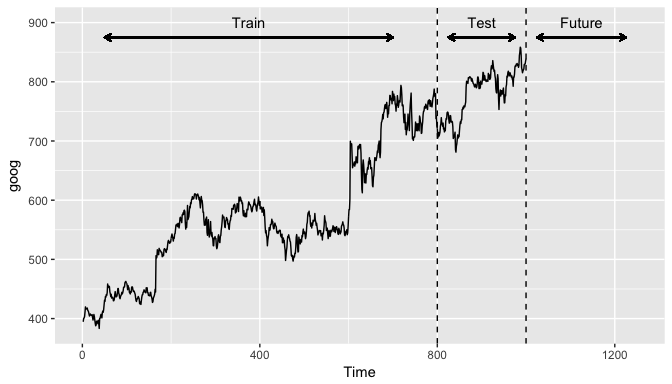
\includegraphics[scale=0.35]{partitioning-1.png}

\emph{Źródło: http://uc-r.github.io/ts\_benchmarking}
\end{figure}
\end{frame}

%--------------------------------------------------------------
\begin{frame}{Jakość prognozy}
\begin{itemize}
    \item Błędy prognozy
    \[
    e_{t}=y_{t}-y_{t}^{f}
    \]
    powinny:
    \begin{itemize}
        \item mieć średnią zero (inaczej prognoza \emph{obciążona}),
        \item być nieskorelowane (inaczej nie wykorzystaliśmy części informacji w~danych).
    \end{itemize}
    \item Pożądane właściwości:
    \begin{itemize}
        \item stała wariancja,
        \item rozkład normalny.
    \end{itemize}
\end{itemize}
\end{frame}

%--------------------------------------------------------------
\begin{frame}{Jakość prognozy}
\begin{itemize}
    \item \textbf{Błąd prognozy ex ante:} opisuje \emph{dopuszczalność} prognozy.
    \begin{itemize}
        \item Przed upływem czasu, na który prognoza była ustalona.
    \end{itemize}
    \item \textbf{Błąd prognozy ex post:} opisuje \emph{trafność} prognozy.
    \begin{itemize}
        \item Można obliczyć, gdy znana jest realizacja zmiennej prognozowanej.
        \item To nimi będziemy się zajmować głównie na tych zajęciach.
    \end{itemize}
\end{itemize}
\end{frame}

%--------------------------------------------------------------
\begin{frame}{Miary błędów ex post}
\small
\begin{itemize}
    \item Notacja: używamy $n$ obserwacji do prognozy na okresy $n+1,n+2,\ldots,T$.
    \item \textbf{MAE} -- mean absolute error
    \[
    \frac{1}{T-n}\sum_{t=n+1}^{T}\left|e_{t}\right|
    \]
    \item \textbf{MSE} -- mean square error
    \[
    \frac{1}{T-n}\sum_{t=n+1}^{T}e_{t}^{2}
    \]
    \item \textbf{RMSE} -- \emph{root} mean square error
    $\displaystyle\sqrt{\frac{1}{T-n}\sum_{t=n+1}^{T}e_{t}^{2}}$
    \item Powyższe \emph{nie} spełniają warunku unormowania (niejasna interpretacja).
\end{itemize}
\end{frame}

%--------------------------------------------------------------
\begin{frame}{Miary błędów ex post}
\begin{itemize}
    \item \textbf{MAPE} -- mean absolute \emph{percentage} error
    \[
    \frac{1}{T-n}\sum_{t=n+1}^{T}\left|\frac{e_{t}}{y_{t}}\right|\times 100\%
    \]
    \item \textbf{AMAPE} -- \emph{adjusted} MAPE
    \[
    \frac{1}{T-n}\sum_{t=n+1}^{T}\left|\frac{e_{t}}{y_{t}+y_{t}^{f}}\right|\times 100\%
    \]
\end{itemize}
\end{frame}

%--------------------------------------------------------------
\begin{frame}{Przedziały}
\begin{itemize}
    \item Często interesuje nas przedział, w którym $y_{t}$ będzie znajdować się z~określonym prawdopodobieństwem.
    \item Na przykład, jeśli założymy że błędy prognozy mają rozkład normalny, to
    \[
    y_{t+h}\in\left[y_{t+h}^{f}-1{,}96\,\hat{\sigma}_{h},\;y_{t+h}^{f}+1{,}96\,\hat{\sigma}_{h}\right]
    \]
    z prawdopodobieństwem $0{,}95$, gdzie $\hat{\sigma}_{h}$ to oszacowanie odch.\ standardowego błędu prognozy o~horyzoncie $h$.
\end{itemize}
\end{frame}

%--------------------------------------------------------------
\begin{frame}{Przedziały}
\begin{itemize}
    \item $\hat{\sigma}_{1}$ można obliczyć szacując odchylenie standardowe reszt.
    \item $\hat{\sigma}_{h}$ zazwyczaj rośnie wraz z~$h$. Obliczenie nieco trudniejsze, zwłaszcza gdy reszty są ze sobą skorelowane.
\end{itemize}
\end{frame}

%--------------------------------------------------------------
\section{Metody naiwne}

\begin{frame}{Metody naiwne}
\begin{itemize}
    \item Najprostszy typ metod wykorzystywanych do prognozowania.
    \item Założenie: brak zmian czynników oddziaływujących na zmienną prognozowaną.
    \begin{itemize}
        \item Stosowane w przypadku niewielkich wahań przypadkowych zmiennej zależnej.
    \end{itemize}
    \item Zazwyczaj niska jakość prognoz.
\end{itemize}
\end{frame}

%--------------------------------------------------------------
\begin{frame}{Metody naiwne}
\begin{itemize}
    \item Najprostsza prognoza naiwna:
    \[
    y_{t}^{f}=y_{t-1}
    \]
    gdzie $y_{t}^{f}$ to prognoza wartości zmiennej zależnej na moment $t$, a~$y_{t-1}$ to faktyczna wartość tej zmiennej w~momencie $t-1$.
    \item Możemy też mieć prognozę z horyzontem $h$:
    \[
    y_{t+h}^{f}=y_{t}
    \]
    \item Co z trendem, sezonowością?
\end{itemize}
\end{frame}

%--------------------------------------------------------------
\begin{frame}{Prognoza naiwna sezonowa}
\begin{itemize}
    \item Jeśli szereg wykazuje sezonowość o~długości cyklu $m$:
    \[
    y_{t+h}^{f}=y_{t+h-m}
    \]
    \item Prognoza powtarza wartość z~\emph{analogicznego} okresu w~ostatnim cyklu.
    \begin{itemize}
        \item Np.\ dla danych miesięcznych ($m=12$): prognoza na styczeń~2026 = wartość ze stycznia~2025.
    \end{itemize}
    \item Ważny \textbf{benchmark} -- jeśli bardziej złożona metoda nie bije prognozy naiwnej sezonowej, to warto się zastanowić, czy jest potrzebna.
\end{itemize}
\end{frame}

%--------------------------------------------------------------
\begin{frame}{Metoda dryfu (\emph{drift})}
\begin{itemize}
    \item Prognoza naiwna z~uwzględnieniem średniego tempa zmian:
    \[
    y_{T+h}^{f}=y_{T}+h\,\frac{y_{T}-y_{1}}{T-1}
    \]
    \item Równoważne poprowadzeniu linii prostej między pierwszą a~ostatnią obserwacją i~ekstrapolowaniu jej w~przyszłość.
    \item Przydatna, gdy szereg wykazuje trend, a~nie chcemy jeszcze stosować bardziej złożonych metod.
\end{itemize}
\end{frame}

%--------------------------------------------------------------
\section{Metody średniej ruchomej}

\begin{frame}{Metody średniej ruchomej}
\begin{itemize}
    \item Wykorzystywane do:
    \begin{itemize}
        \item \textbf{wygładzania} szeregu czasowego (X11/X12/X13),
        \item \textbf{prognozowania} -- prognozowana wartość zmiennej to średnia z~$k$ poprzednich obserwacji.
    \end{itemize}
\end{itemize}
\end{frame}

%--------------------------------------------------------------
\begin{frame}{Metody średniej ruchomej -- wygładzanie}
\[
y_{t}^{s}=\frac{1}{2n+1}\sum_{i=-n}^{n}y_{t-i}
\]
gdzie $y_{t}^{s}$ to wartość zmiennej w~okresie $t$ po wygładzaniu \emph{(smoothed)}, a~$y_{t-n},y_{t-n+1},\ldots,y_{t+n}$ to faktyczne wartości zmiennej.
\begin{itemize}
    \item Do wygładzania używamy obserwacji w~okresie $t$ oraz $n$ poprzedzających i~$n$ kolejnych obserwacji.
    \item Częste oznaczenie: $k=2n+1$ ($k$ to \emph{stała wygładzania szeregu}).
\end{itemize}
\end{frame}

%--------------------------------------------------------------
\begin{frame}{Metody średniej ruchomej -- prognozowanie}
\[
y_{t}^{f}=\frac{1}{k}\sum_{i=t-k}^{t-1}y_{i}
\]
gdzie $y_{t}^{f}$ to prognozowana wartość zmiennej w~okresie $t$, a~$y_{t-k},y_{t-k+1},\ldots,y_{t-1}$ to faktyczne wartości zmiennej.
\begin{itemize}
    \item Do prognozowania używamy obserwacji w~okresie $t-1$ oraz $k-1$ poprzedzających obserwacji.
    \item Dla $k=1$ sprowadza się do metody naiwnej.
\end{itemize}
\end{frame}

%--------------------------------------------------------------
\begin{frame}{Jak wybrać $k$?}
\begin{itemize}
    \item Jakie $k$ jest najlepsze?
    \item Pomysł: jak dobrze prognozujemy dane, które zaobserwowaliśmy?
    \begin{itemize}
        \item Błąd prognozy \textbf{\emph{ex post}}.
    \end{itemize}
    \item Szukamy $k$, które minimalizuje
    \[
    MSE_{k} \coloneqq \frac{1}{T-k}\sum_{t=k+1}^{T}\left(y_{t}-y_{t}^{f}\right)^{2}
    \]
\end{itemize}
\end{frame}

%--------------------------------------------------------------
\begin{frame}{Ważona średnia ruchoma}
\begin{itemize}
    \item Obserwacje starsze mają mniejsze znaczenie:
    \[
    y_{t}^{f}=\sum_{i=1}^{k}w_{i}\,y_{t-k+i-1}
    \]
    gdzie
    \begin{align*}
    \sum_{i=1}^{k}w_{i} &= 1\\
    0<w_{1}<w_{2}<\cdots<w_{k} &\leq 1
    \end{align*}
\end{itemize}
\end{frame}

%--------------------------------------------------------------
\section{Metody wygładzania wykładniczego}

\begin{frame}{Proste wygładzanie wykładnicze}
\begin{itemize}
    \item Stosowane w przypadku braku trendu i sezonowości:
    \[
    y_{t}^{f}=\alpha\, y_{t-1}+\left(1-\alpha\right)y_{t-1}^{f}
    \]
    alternatywnie
    \[
    y_{t}^{f} = y_{t-1}^{f}+\alpha\left(y_{t-1}-y_{t-1}^{f}\right)
    \]
\end{itemize}
\end{frame}

%--------------------------------------------------------------
\begin{frame}{Proste wygładzanie wykładnicze}
\begin{itemize}
    \item Skąd nazwa?
    \begin{align*}
    y_{t}^{f} &= \alpha\, y_{t-1}+\left(1-\alpha\right)y_{t-1}^{f}\\
     &= \alpha\, y_{t-1}+\left(1-\alpha\right)\!\left[\alpha\, y_{t-2}+\left(1-\alpha\right)y_{t-2}^{f}\right]\\
     &= \alpha\, y_{t-1}+\alpha\left(1-\alpha\right)y_{t-2}+\left(1-\alpha\right)^{2}y_{t-2}^{f}\\
     &= \alpha\, y_{t-1}+\alpha\left(1-\alpha\right)y_{t-2}+\alpha\left(1-\alpha\right)^{2}y_{t-3}+\cdots
    \end{align*}
    \item Coraz mniejsze wagi przeszłych obserwacji.
\end{itemize}
\end{frame}

%--------------------------------------------------------------
\begin{frame}{Proste wygładzanie wykładnicze}
\begin{itemize}
    \item Jak wybrać $\alpha$?
    \item Najczęściej $\alpha\in\left[0{,}2;\;0{,}3\right]$. Niższa wartość = dłuższa pamięć.
    \begin{itemize}
        \item Dla $\alpha=0$ mamy $y_{t}^{f}=y_{t-1}^{f}$.
        \item Dla $\alpha=1$ mamy $y_{t}^{f}=y_{t-1}$.
    \end{itemize}
    \item Za $y_{1}^{f}$ podstawia się $y_{1}$ lub średnią z kilku pierwszych obserwacji.
    \item W przypadku występowania trendu stosowane \textbf{podwójne} wygładzanie wykładnicze.
\end{itemize}
\end{frame}

%--------------------------------------------------------------
\begin{frame}{Podwójne wygładzanie wykładnicze -- metoda Holta}
\begin{itemize}
    \item Poziom + trend.
    \[
    y_{t-1+k}^{f}=L_{t-1}+k\,T_{t-1}
    \]
    gdzie poziom to
    \[
    L_{t}=\alpha\, y_{t}+\left(1-\alpha\right)\!\left(L_{t-1}+T_{t-1}\right)
    \]
    a trend to
    \[
    T_{t}=\beta\left(L_{t}-L_{t-1}\right)+\left(1-\beta\right)T_{t-1}
    \]
\end{itemize}
\end{frame}

%--------------------------------------------------------------
\begin{frame}{Podwójne wygładzanie wykładnicze -- metoda Holta}
\begin{itemize}
    \item Równanie prognozy na okres $t>T$:
    \[
    y_{t}^{f}=L_{T}+\left(t-T\right)T_{T}
    \]
    gdzie:
    \begin{itemize}
        \item $y_{t}^{f}$ -- prognoza zmiennej wyznaczona na moment $t$,
        \item $L_{T}$ -- wygładzona wartość zmiennej prognozowanej na okres $T$,
        \item $T_{T}$ -- wygładzona wartość przyrostu trendu na okres $T$,
        \item $T$ -- liczba obserwacji zmiennej prognozowanej.
    \end{itemize}
\end{itemize}
\end{frame}

%--------------------------------------------------------------
\begin{frame}{Podwójne wygładzanie wykładnicze -- metoda Holta}
\begin{itemize}
    \item W przypadku metody Holta mamy:
    \begin{align*}
    L_{t} &= y_{t}^{f}+\alpha\left(y_{t}-y_{t}^{f}\right)\\
    T_{t} &= T_{t-1}+\alpha\beta\left(y_{t}-y_{t}^{f}\right)\\
    y_{t}^{f} &= L_{t-1}+T_{t-1}
    \end{align*}
\end{itemize}
\end{frame}

%--------------------------------------------------------------
\begin{frame}{Tłumiony trend (\emph{damped trend})}
\begin{itemize}
    \item Problem metody Holta: prognozy długoterminowe rosną (lub maleją) w~nieskończoność.
    \item Rozwiązanie -- parametr tłumienia $\phi\in(0,1]$:
    \[
    y_{T+h}^{f}=L_{T}+\left(\phi+\phi^{2}+\cdots+\phi^{h}\right)T_{T}
    \]
    \begin{align*}
    L_{t} &= \alpha\, y_{t}+\left(1-\alpha\right)\!\left(L_{t-1}+\phi\, T_{t-1}\right)\\
    T_{t} &= \beta\left(L_{t}-L_{t-1}\right)+\left(1-\beta\right)\phi\, T_{t-1}
    \end{align*}
    \item Dla $\phi=1$ sprowadza się do metody Holta.
    \item Dla $h\to\infty$: $\phi+\phi^{2}+\cdots\to\frac{\phi}{1-\phi}$, więc prognoza zbiega do stałej.
\end{itemize}
\end{frame}

%--------------------------------------------------------------
\begin{frame}{Addytywny model Wintersa}
\begin{itemize}
    \item Poziom + trend + sezonowość.
    \begin{align*}
    y_{t-1+k}^{f} &= L_{t-1}+k\,T_{t-1}+S_{t-1+k-m(z+1)}\\
    L_{t} &= \alpha\left(y_{t}-S_{t-m}\right)+\left(1-\alpha\right)\!\left(L_{t-1}+T_{t-1}\right)\\
    T_{t} &= \beta\left(L_{t}-L_{t-1}\right)+\left(1-\beta\right)T_{t-1}\\
    S_{t} &= \gamma\left(y_{t}-L_{t-1}-T_{t-1}\right)+\left(1-\gamma\right)S_{t-m}
    \end{align*}
    gdzie $m$ oznacza długość cyklu sezonowego (np.\ 4 albo 12), a~$z=\lfloor(k-1)/m\rfloor$.
\end{itemize}
\end{frame}

%--------------------------------------------------------------
\begin{frame}{Multiplikatywny model Wintersa}
\begin{itemize}
    \item Poziom + trend $\times$ sezonowość.
    \begin{align*}
    y_{t-1+k}^{f} &= \left(L_{t-1}+k\,T_{t-1}\right)\times S_{t-1+k-m(z+1)}\\
    L_{t} &= \alpha\!\left(\frac{y_{t}}{S_{t-m}}\right)+\left(1-\alpha\right)\!\left(L_{t-1}+T_{t-1}\right)\\
    T_{t} &= \beta\left(L_{t}-L_{t-1}\right)+\left(1-\beta\right)T_{t-1}\\
    S_{t} &= \gamma\!\left(\frac{y_{t}}{L_{t-1}+T_{t-1}}\right)+\left(1-\gamma\right)S_{t-m}
    \end{align*}
    gdzie $m$ oznacza długość cyklu sezonowego (np.\ 4 albo 12), a~$z=\lfloor(k-1)/m\rfloor$.
\end{itemize}
\end{frame}

%--------------------------------------------------------------
\begin{frame}{Dobór parametrów wygładzania}
\begin{itemize}
    \item Analogicznie do wyboru $k$ w~średniej ruchomej, parametry $\alpha$, $\beta$, $\gamma$ (i~ewentualnie $\phi$) dobieramy minimalizując błąd prognozy \emph{ex post}:
    \[
    \min_{\alpha,\beta,\gamma}\;\frac{1}{T-1}\sum_{t=2}^{T}e_{t}^{2}
    \qquad\text{gdzie}\quad e_{t}=y_{t}-y_{t}^{f}
    \]
    \item Problem optymalizacji nieliniowej -- rozwiązywany numerycznie (np.~funkcja \texttt{ets()} w~R).
    \item Ograniczenia: $\alpha,\beta,\gamma\in(0,1)$, $\phi\in(0{,}8;\;1)$.
    \item Uwaga: optymalne $\alpha$ na zbiorze treningowym nie gwarantuje najlepszej prognozy poza próbą -- stąd rola zbioru testowego.
\end{itemize}
\end{frame}

\end{document}
